\documentclass{article} % For LaTeX2e
\usepackage{nips14submit_e,times}
\usepackage{hyperref}
\usepackage{url}
%\documentstyle[nips14submit_09,times,art10]{article} % For LaTeX 2.09

\usepackage{graphicx}
\usepackage{subfigure}
\usepackage{amsmath,amssymb}
\def\etal{{\textit{et~al.~}}}

\title{Exploiting Linear Structure Within Convolutional Networks
  for Efficient Evaluation}


\author{
Emily Denton$^1$, Wojciech Zaremba$^1$, Joan Bruna$^1$, Yann LeCun$^{12}$ and Rob Fergus$^{12}$\\\\
$^1$New York University\\
$^2$Facebook AI Group\\\\
\texttt{ \{denton, zaremba, bruna, lecun, fergus\} @cs.nyu.edu} \\
}

% The \author macro works with any number of authors. There are two commands
% used to separate the names and addresses of multiple authors: \And and \AND.
%
% Using \And between authors leaves it to \LaTeX{} to determine where to break
% the lines. Using \AND forces a linebreak at that point. So, if \LaTeX{}
% puts 3 of 4 authors names on the first line, and the last on the second
% line, try using \AND instead of \And before the third author name.

\newcommand{\fix}{\marginpar{FIX}}
\newcommand{\new}{\marginpar{NEW}}

%\nipsfinalcopy % Uncomment for camera-ready version

\begin{document}


\maketitle

\begin{abstract}
  We present techniques for speeding up the test-time evaluation of
  large convolutional networks, designed for object recognition
  tasks. These models deliver impressive accuracy but each image
  evaluation requires millions of floating point operations, making
  their deployment on smartphones and Internet-scale clusters
  problematic. The computation is dominated by the convolution
  operations in the lower layers of the model. We exploit the linear
  structure present within the convolutional filters to derive
  approximations that significantly reduce the required
  computation. Using large state-of-the-art models, we demonstrate
  speedups by a factor of $2\times$, while keeping the accuracy
  within $1\%$ of the original model.
\end{abstract}

\section{Introduction}

Large neural networks have recently demonstrated impressive
performance on a range of speech and vision tasks. However the size of
these models can make their deployment at test time problematic. For
example, mobile computing platforms are limited in their CPU speed,
memory and battery life. At the other end of the spectrum,
Internet-scale deployment of these models requires thousands of
servers to process the 100's of millions of images per day. The
electrical and cooling costs of these servers required is significant.

Training large neural networks can take weeks, or even
months. This hinders research and consequently there have been
extensive efforts devoted to speeding up training procedure.  However,
there are relatively few efforts aimed at improving the {\em test-time}
performance of the models. 

In this paper we focus on speeding up the evaluation of {\em trained}
networks, with minimal compromise to performance. We consider
convolutional neural networks used for computer vision tasks, since
they are large and widely used in commercial applications. Within
these models, most of the time ($\sim90\%$) is spent in the
convolution operations in the lower layers of the model. The remaining
operations: pooling, contrast normalization and the upper
fully-connected layers collectively take up the remaning $10\%$.

We present several novel methods for speeding up the convolution
operations. They are based on various low-dimensional approximations of convolution
operators (which are 4-dimensional tensors), and exploit sparsity to
deliver speedups in performance. Viability of methods is architecture 
dependent, and speedup by factor of $2$ is quite achievable without fine-tuning.
However, a much larger speedup should be attainable if the models were
trained for a few more epochs after imposing the filter approximation.

Neural networks are stacked linear transforms alternated with simple
point-wise non-linearities. From mathematical perspective, we have a good understanding
of linear operators, however properties of composed operators are much more
difficult to understand. Our studies of filter compressibility reveal some of underlying
low-dimensional structure. Effectively, it decreases number of parameters, and
potentially might lead to better model generalization if used during training.
We observe some indications that it is indeed feasible. In particular,
the first layer filters look ``cleaner'' after approximation and can,
on occasion, yield a slightly lower test error than the original versions,
provided the approximations are mild. 

\section{Related Work}

Vanhoucke \etal \cite{vanhoucke2011improving} explored the
properties of CPUs to speed up execution.  They present many solutions
specific to Intel and AMD CPUs, however some of their techniques are
general enough to be used for any type of processor.  They describe
how to align memory, and use SIMD operations (vectorized operations on
CPU) to boost the efficiency of matrix multiplication.  Additionally, they
propose the linear quantization of the network weights and input. This
involves representing weights as 8-bit integers (range
$[-127, 128]$), rather than 32-bit floats. This approximation is
similar in spirit to our approach, but differs in that it is applied
to each weight element independently. By contrast, our approximation approach models
the structure within each filter. Potentially, the two approaches
could be used in conjunction. 


The most expensive operations in convolutional networks are the
convolutions in the first few layers. The complexity of this operation
is linear in the area of the receptive field of the filters, which is
relatively large for these layers.  However, Mathieu \etal \cite{mathieu2013fast} have shown that convolution can be
efficiently computed in Fourier domain, where it becomes element-wise
multiplication (and there is no cost associated with size of receptive
field). They report a forward-pass speed up of around $2\times$ for
convolution layers in state-of-the-art models. Importantly, the FFT method can
be used jointly with most of techniques presented in this paper.

The use of low-rank approximations in our approach is inspired by work
of Denil \etal \cite{denil2013predicting} who demonstrate the redundancies in neural
network parameters. They show that the weights within a layer can be
accurately predicted from a small (e.g. $\sim 5\%$) subset of them. This
indicates that neural networks are heavily over-parametrized.  All the
methods presented here focus on exploiting the linear structure of this
over-parametrization.

\section{Tensor Approximation Techniques}\label{sec:approx_tech}
In typical object recognition architectures, the weights of
convolutional layers at the end of training exhibit strong redundancy
and regularity across all dimensions. In this section we describe
techniques then can be used to exploit this structure to compress the
4 dimensional weight tensors into a representation that permits
efficient computation. 

Section \ref{subsec:low_rank} reviews techniques for low-rank tensor
approximations,
Section \ref{subsec:clustering} shows how to use clustering algorithms to
discover, and later exploit, patterns between input and output
features.

 \vspace{2mm}

 \noindent \textbf{Notation:} Convolution weights can be described as
 a $4$-dimensional tensor: $W \in \mathbb{R}^{C \times X \times Y
   \times F}$. $C$ is the number of number of input channels, $X$ and
 $Y$ are the spatial dimensions of the kernel, and $F$ is the target
 number of feature maps. It is common for the first convolutional layer to have a stride associated with the kernel. We denote the stride by $\Delta$.  Let $I \in \mathbb{R}^{C \times N \times M}$
 denote an input signal where $C$ is the number of input maps, and $N$
 and $M$ are the spatial dimensions of the maps.  The target value, $T
 = I \ast W$, of a generic convolutional layer, with $\Delta = 1$, for a particular output
 feature, $f$, and spatial location, $(x, y)$, is defined as
\begin{align*}
\label{convlayereq}
T(f,x,y) = \sum_{c=1}^C \sum_{x'=1}^{X} \sum_{y'=1}^{Y} I(c,x+x',y+y') W(c,x',y',f)
\end{align*}

Moreover, we define $W_C \in \mathbb{R}^{C \times (XYF)}$, and $W_F \in \mathbb{R}^{(CXY) \times F}$, 
and $W_S \in \mathbb{R}^{C \times (XY) \times F}$ to be the folded, with respect to different dimensions, versions of $W$.

\vspace{-0.3cm}
\subsection{Low-rank Approximations}\label{subsec:low_rank}
A particularly simple way to exploit the regularity present in trained convolutional network weights is to linearly compress the tensors, which amounts to finding low-rank approximations. In this section we describe two different techniques for expressing matrices and tensors as a product of matrices or vectors of smaller size. 

\vspace{-0.3cm}
\subsubsection{Singular Value Decomposition for Matrices:}\label{subsubsec:svd}
Let $I \in \mathbb{R}^{n \times m}$ denote the input to a fully connected layer of a neural network and let $W \in \mathbb{R}^{m \times k}$ denote the weight matrix for the layer. Matrix multiplication,  the main operation for fully connected layers, costs $O(nmk)$. However, $W$ is likely to have a low-rank structure and thus have several eigenvalues close to zero. These dimensions can be interpreted as noise, and thus can be eliminated without harming the accuracy of the network. We now show how to exploit this low-rank structure to compute $IW$ much faster than $O(nmk)$. 


Every matrix $W \in \mathbb{R}^{m \times k}$ can be expressed using singular value decomposition:
\begin{equation*}
	W = USV^{\top}\text{, where }U \in \mathbb{R}^{m \times m}, S \in \mathbb{R}^{m \times k}, V \in \mathbb{R}^{k \times k}
\end{equation*}
$S$ is a diagonal matrix with  singular value on the diagonal, and U, V are orthogonal matrices. If the singular values of $W$ decay rapidly, $W$ can be well approximated by keeping only the $t$ largest singular values from $S$. We can write the approximation as
\begin{equation}
\label{svdapprox}
	\tilde{W} = \tilde{U}\tilde{S}\tilde{V}^{\top}\text{, where }\tilde{U} \in \mathbb{R}^{m \times t}, \tilde{S} \in \mathbb{R}^{t \times t}, \tilde{V} \in \mathbb{R}^{t \times k}
\end{equation}
The approximation error $\| I \tilde{W} - I W \|_F$ satisfies 
\begin{equation}
\label{svdapproxerr}
\| I \tilde{W} - I W \|_F \leq S(t+1,t+1) \| I \|_F~,
\end{equation}
and thus is controlled by the decay along the diagonal of $S$.
Now the computation $I\tilde{W}$ can be done in $O(nmt + nt^2 + ntk)$, which, for sufficiently small $t$ is significantly smaller than $O(nmk)$. 

\vspace{-0.3cm}
\subsubsection{Singular Value Decomposition for Tensors:}\label{subsubsec:svd_tensor}
Any tensor can be converted to a matrix by folding all but two
dimensions together.  For example, let $W_C \in \mathbb{R}^{C \times (XYF)}$ be a folded version of $W$ where the spatial and output dimensions have been folded together. Singular value decomposition of
$W_C$ can decrease number of input colors on which the convolution has to
operate in exchange for an additional matrix multiplication
operation. More formally, $$W_C = USV^T \approx
\tilde{U}\tilde{S}\tilde{V}^T$$
 $\tilde{U}\tilde{S}$ is a matrix that
transforms input colors to intermediate output.  Then $\tilde{V}$ is
considered as convolution operator on intermediate output space. 
Similarly, we can apply SVD to $W_F \in \mathbb{R}^{(CXY) \times F}$ or $\tilde{V}$. 

\vspace{-0.3cm}
\subsubsection{Outer Product Decomposition for Tensors:}\label{subsubsec:outer}
The linear approximation of matrices can be easily extended to higher order tensors.
Let $v \otimes l$ denote the outer product.
For a 3-tensor, $W_S \in \mathbb{R}^{C \times (XY) \times F}$, we can construct a rank $1$ approximation by finding a decomposition that minimizes 
\begin{equation}
\label{eq:rank1}
	\| W_S - \alpha \otimes \beta \otimes \gamma \|_F~,
\end{equation} 
where $\alpha \in \mathbb{R}^C$, $\beta \in \mathbb{R}^{XY}$, $\gamma \in \mathbb{R}^F$ and $\|X\|_F$ denotes the Frobenius norm.
Problem (\ref{eq:rank1}) is solved efficiently by performing alternate least squares 
on $\alpha$, $\beta$ and $\gamma$ respectively. 

This easily extends to a rank $K$ approximation using a greedy algorithm: Given a 
tensor $M$, we compute $(\alpha, \beta, \gamma)$ using (\ref{eq:rank1}), and we update 
$W_S \leftarrow W_S - \alpha \otimes \beta \otimes \gamma$. Repeating this operation $K$
times results in 
\begin{equation}
\label{eq:rankK}
	\tilde{W_S} = \sum_{k = 1}^{K} \alpha_k \otimes \beta_k \otimes \gamma_k ~.
\end{equation} 
where $\alpha \in \mathbb{R}^C$, $\beta \in \mathbb{R}^{XY}$, $\gamma \in \mathbb{R}^F$ 

The approximations (\ref{eq:rank1}) and (\ref{eq:rankK}) are extended to $q$-tensors 
by adding more terms in the separable approximations.
As opposed to the SVD for matrices, the rank-1 tensors are not orthogonal in general. 


\subsection{Clustering}\label{subsec:clustering}
Another form of structure within the 4-D weight tensors that can be exploited is the similarity between different filters. 
We can capture this by first splitting the filters into groups and then approximating the weights within a group using a low-rank factorization method.  
We found it to be most efficient to independently cluster
over both input and output feature channels. We start by clustering the
rows of $W_C \in \mathbb{R}^{C \times (XYF)}$, which results in
clusters $C_1, \dots, C_a$. Then we cluster the columns of $W_F  \in
\mathbb{R}^{(CXY) \times F}$. This procedure returns clusters $F_1,
\dots, F_b$. These two operations break the original weight tensor $W$
into $ab$ sub-tensors $\{W_{C_i, F_j}\}_{i = 1, \dots, a, j = 1,
  \dots, b}$ as shown in Figure \ref{fig:biclustering}). Each
sub-tensor contains similar elements making this approach more
efficient than attempting to fit a low rank approximation to all
filters.

In order to efficiently exploit the parallelism inherent in CPU and GPU
architectures it is useful to constrain clusters to be of equal sizes. 
We therefore perform the biclustering operations (or clustering 
for monochromatic filters \ref{subsec:monochromatic}) using a modified
version of the k-means algorithms which balances the cluster count at
each iteration
It is implemented with the Floyd algorithm, by modifying the Euclidean distance
with a subspace projection distance.

\section{Application to Convolutional Networks}\label{sec:application}
In this section we describe how to use the techniques described in
Section \ref{sec:approx_tech} to approximate covolutional weight
tensors in ways that allow for a more efficient computation of the
convolution. The approximations are more efficient in two senses:
both the number of floating point operations required to compute the
convolution output and the number of parameters that need to be stored
are dramatically reduced.

The first convolutional layer in the standard architecture receives
three color channels, typically in RGB or YUV space, as input whereas
later hidden layers typically receive a much larger number of feature
maps that have resulted from computations performed in previous
layers. As a result, the first layer weights often have a markedly
different structure than the weights in later convolutional layers. We
have found that different approximation techniques are well suited to
the different layers. The first approach, which we call {\em monochromatic
approximation}, can be applied to the weights in the first
convolutional layer. For the remaining layers, where the number of
input and output maps are large, we use the 
biclustering approximation, outlined in Section
\ref{subsubsec:biclustering}.

We will compare the number of floating-point operations for different
approximation methods. Table \ref{table:ops} shows a breakdown of the number of operations required for the standard convolution and for our approximations.

\begin{figure}[ht]
\centering
\mbox{
\hspace{5mm}
\subfigure[][]{
  \includegraphics[width=0.4\linewidth]{img/monochromatic_illustration.pdf} 
  \label{fig:monochromatic}
}
\hspace{5mm}
\subfigure[][]{
  \includegraphics[width=0.35\linewidth]{img/bicluster_illustration.pdf} 
  \label{fig:biclustering}
}
}
\vspace{-3mm}
\caption{ A visualization of monochromatic and biclustering approximation structures. {\bf (a)}: The monochromatic approximation, used for the first layer. Input color channels are projected by a set of intermediate color channels. After this transformation, output features need only to look at one intermediate color channel. This sparsity structure is what makes the speedups feasible. {\bf (b)}: The biclustering approximation, used for higher convolution layers. Input and output features are clustered into equal sized groups. The weight tensor corresponding to each pair of input and output clusters is then approximated.}
\end{figure}

\subsection{Monochromatic Approximation}\label{subsec:monochromatic}
Let $W \in \mathbb{R}^{C \times X \times Y \times F}$ denote the
weights of the first convolutional layer of a trained network.  The
number of input channels, $C$, corresponds to a different color
component (either RGB or YUV).  We found that the color components of trained convolutional neural networks we considered (see
section \ref{sec:experiments}) tend to have low dimensional structure. In
particular, the weights can be well approximated by projecting the
color dimension down to a 1D subspace, i.e. a single color
channel. The low-dimensional structure of the weights is apparent in
\ref{fig:RGB_components}. This figure shows the original first layer convolutional weights
of a trained network and the weights after the color dimension has
been projected into 1D lines.


The monochromatic approximation exploits this structure and is computed as follows.
First, for every output feature, $f$, we consider consider the matrix $W_f \in \mathbb{R}^{C \times (X\cdot Y) }$, 
where the spatial dimensions of the filter corresponding to the output feature have been combined, and find the singular value decomposition, 
\begin{equation*}
	W_f = U_f S_f V_f^{\top}
\end{equation*}
where $U_f \in \mathbb{R}^{C \times C}, S_f \in \mathbb{R}^{C \times XY}, V_f \in \mathbb{R}^{XY \times XY}$. 
We then take the rank 1 approximation to $W_f$ 
\begin{equation}
\label{blo1}
	\tilde{W}_f = \tilde{U}_f \tilde{S}_f \tilde{V}_f^{\top}
\end{equation}
where $\tilde{U}_f \in \mathbb{R}^{C \times 1}, \tilde{S}_f \in \mathbb{R}, \tilde{V}_f \in \mathbb{R}^{1 \times XY}$.

This approximation corresponds to shifting from $C$ color channels to $1$ color channel for each output feature. 
We can further exploit the regularity in the weights by sharing the color component basis between different output features. 
We do this by clustering the $F$ left singular vectors, $\tilde{U}_f$, of each output feature $f$ into $C'$ clusters, 
where $C'$ is much smaller than $F$. We constrain the clusters to be of equal size as discussed in section \ref{subsubsec:biclustering}.  
Then, for each of the $\frac{F}{C'}$ output features $f$ that is assigned to cluster $c_f$, we can approximate $W_f$ with
\begin{equation}
\label{blo2}
	\tilde{W}_f = U_{c_f} \tilde{S}_f \tilde{V}_f^{\top}
\end{equation}
where $U_{c_f} \in \mathbb{R}^{C \times 1}$ is the cluster center for cluster $c_f$ and $\tilde{S}_f$ and $\tilde{V}_f$ as as before. 


By decomposing the approximated weights into two tensors, this low-rank approximation
 allows for a more efficient computation of the convolutional layer output. 
 Let $W_C \in \mathbb{R}^{C' \times C}$ denote the color transform matrix 
 where the rows of $W_C$ are the cluster centers $U_c^{\top}$. 
 Let $W_{mono} \in \mathbb{R}^{X \times Y \times F}$ denote the monochromatic 
 weight tensor containing $ \tilde{S}_f \tilde{V}_f^{\top}$ for each of the $F$ output features. 
 Given this decomposition, we can compute the output of the convolutional layer by first 
 transforming the input signal, $I \in \mathbb{R}^{C \times N \times M}$ into a different 
 basis using the color transform matrix: $\tilde{I} = W_C \otimes I$
 where $\tilde{I} \in \mathbb{R}^{C' \times N \times M}$. 

After the color transformation (left part of the Figure \ref{fig:monochromatic}), 
each of the $f$ filters in $W_{mono}$ is monochromatic in the sense that it only acts upon one of the $C'$ color channels 
(right part of the Figure \ref{fig:monochromatic}). 
The fact that this approximation can be made without hurting performance indicates that the 
structure inherent in first layer weights inherently has sparsity
between the input and output maps, when projected into the new color basis. 
If the color transformation is computed once at the outset, then the
number of operations performed is significantly reduced. Table \ref{table:ops} shows the number of operations required for the standard and monochromatic versions.

\subsection{Biclustering Approximations}
The number of  input and output feature planes is large for all layers
beyond the first. As described in Section
\ref{subsubsec:biclustering} we cluster input and output features and then, for each input-output pair,approximate the resulting sub-tensor separately. We explore two different approximations
for each sub-tensor: (i) SVD (see Section \ref{subsubsec:svd_tensor}),
and (ii) outer product decomposition (see Section \ref{subsubsec:outer}).

Using these approximations on the convolutional weights, the target
output can be computed with significantly fewer operations. The number
of operations required is a function of both the number
of input clusters, $G$, and output clusters $H$.  Moreover, let $K$ denote the
rank of the approximated tensors for the outer product decomposition.
For the SVD decomposition, let $K_1$ denote the input mapping rank, and let $K_2$ denote the output mapping rank. The two different approximation methods have the following number of
operations:

\begin{table}[t]
\tiny
\centering
\begin{tabular}{lc}
\hline
Approximation technique & Number of operations \\
\hline
No approximation & $X Y C F N M \Delta^{-2}$\\
Monochromatic & $C' C N M + X Y F N M \Delta^{-2}$\\
Biclustering + outer product decomposition & $G H K (N M \frac{C}{G} + X Y N M \Delta^{-2} + \frac{F}{H} N M \Delta^{-2})$ \\  
Biclustering + SVD & $G H N M (\frac{C}{G}K_1 + K_1 X Y K_2 \Delta^{-2} + K_2\frac{F}{H})$\\
\end{tabular}
\caption{Number of operations required for verious approximation methods.} 
\label{table:ops}
\end{table}



%Some ways of addressing it : 
%- Global approximation based on :
%	- backpropagation 
%	- Hessian
%- Local approximation : 
%	- relate to work of Simoncelli 


\section{Experiments}\label{sec:experiments}

We use the convolutional architecture of \cite{zeiler2013visualizing}, trained on the
ImageNet 2012 dataset \cite{imagenet}.
We evaluate these networks on both CPU and GPU platforms. All measurements of prediction performance are with respect to the 20K validation images from the ImageNet12 dataset. 

We present results showing the performance of the approximations described in section \ref{sec:approx_tech} in terms of prediction accuracy, speedup gains and reduction in memory overhead. 

\subsection{Speedup}
The majority of forward propagation time is spent on the first two convolutional layers (see Supplementary Material for breakdown of time across all layers).
Because of this, we restrict our attention to the first and second convolutional layers in our speedup experiments. 
However, our approximations could easily
applied to convolutions in upper layers as well.

We implemented several different CPU and GPU approximation routines 
in an effort to achieve empirical
speedups. Both the baseline and approximation CPU code is implemented
in C++ using Eigen3 library \cite{eigenweb} compiled with Intel MKL.
We also use Intel's implementation of openmp and multithreading. The
baseline gives comparable performance to highly optimized MATLAB
convolution routines and all of our CPU speedup results are computed
relative to this.  We used Alex Krizhevsky's CUDA convolution routines
\footnote{\url{https://code.google.com/p/cuda-convnet/}} as a baseline for GPU
comparisons. The approximation versions are written in CUDA. All GPU
code was run on a standard nVidia Titan card.

We have found that in practice it is often difficult to achieve
speedups close to the theoretical gains based on the number of
arithmetic operations (see Supplementary Material for discussion of theoretical gains).
Moreover, different computer architectures and convolutional network
architectures afford different optimization strategies making most
implementations highly specific.  However, regardless of
implementation details, all of the approximations we present reduce
both the number of operations and number of weights required to
compute the output by at least a factor of two, often more.  

\subsubsection{First Layer}

The first convolutional layer has 3 input channels, 96
output channels and 7x7 filters.  We approximated the weights in this
layer using the monochromatic approximation described in section
\ref{subsec:monochromatic}. The monochromatic approximation works well if
the color components span a small number of one dimensional
subspaces. Figure \ref{fig:RGB_components} illustrates the effect of the monochromatic approximation on the first layer filters. 
Interestingly, we
notice that the approximated filters often appear to be cleaned up
versions of the original filters. This leads up to believe that the
approximation techniques presented here might be viable strategies of
cleaning up or denoising weights after training, potentially improving generalization performance.

\begin{figure}[t]
\centering
\begin{minipage}{\textwidth}
	\includegraphics[width=0.5\linewidth]{img/RGB_components_stacked.pdf}
	\includegraphics[width=0.5\linewidth]{img/denoised_stacked.pdf} 
\end{minipage}
\vspace{-3mm}
\label{fig:RGB_components}
\caption{Visualization of the 1st layer filters. Each component of the 96 7x7 filters is plotted in RGB space. Points are colored based on the output filter they belong to. Hence, there are 96 colors and $7^2$ points of each color. {\bf (Left)} Shows the
  original filters and {\bf (Middle)} shows the filters after the monochromatic approximation, where each filter has been projected down to a line in colorspace. {\bf (Right)} Original and approximate versions of a selection of 1st layer filters.}
\end{figure}

We evaluated the network on 20K validation images from the ImageNet12 dataset using various monochromatic approximations for the first layer weights. 
The only parameter in the approximation is $C'$, the number of color channels used for the intermediate representation. As expected, the network performance begins to degrade as $C'$ decreases. 

The number of FLOPS required to compute the output of the monochromatic convolution is reduced by a factor of $2-3\times$, with the larger gain resulting for small $C'$. 
Since the majority of the operations result from the convolution part of the computation, rather than the color transform,
the theoretically achievable speedup decreases only slightly as $C'$ is increased.
In practice, we found it difficult to optimize the monochromatic convolution routines as for large $C'$ since less work can be shared amongst output filters making it challenging to parallelize.
Figure \ref{fig:mono_speedups} shows the empirical speedups we achieved on CPU and GPU and the corresponding network performance for various numbers of colors used in the monochromatic approximation.   
Our CPU and GPU implementations achieve empirical speedups of $2-2.5\times$ relative to the baseline with less than 1\% drop in classification performance. 

\begin{figure}[t]
\centering
\begin{minipage}{0.9\textwidth}
      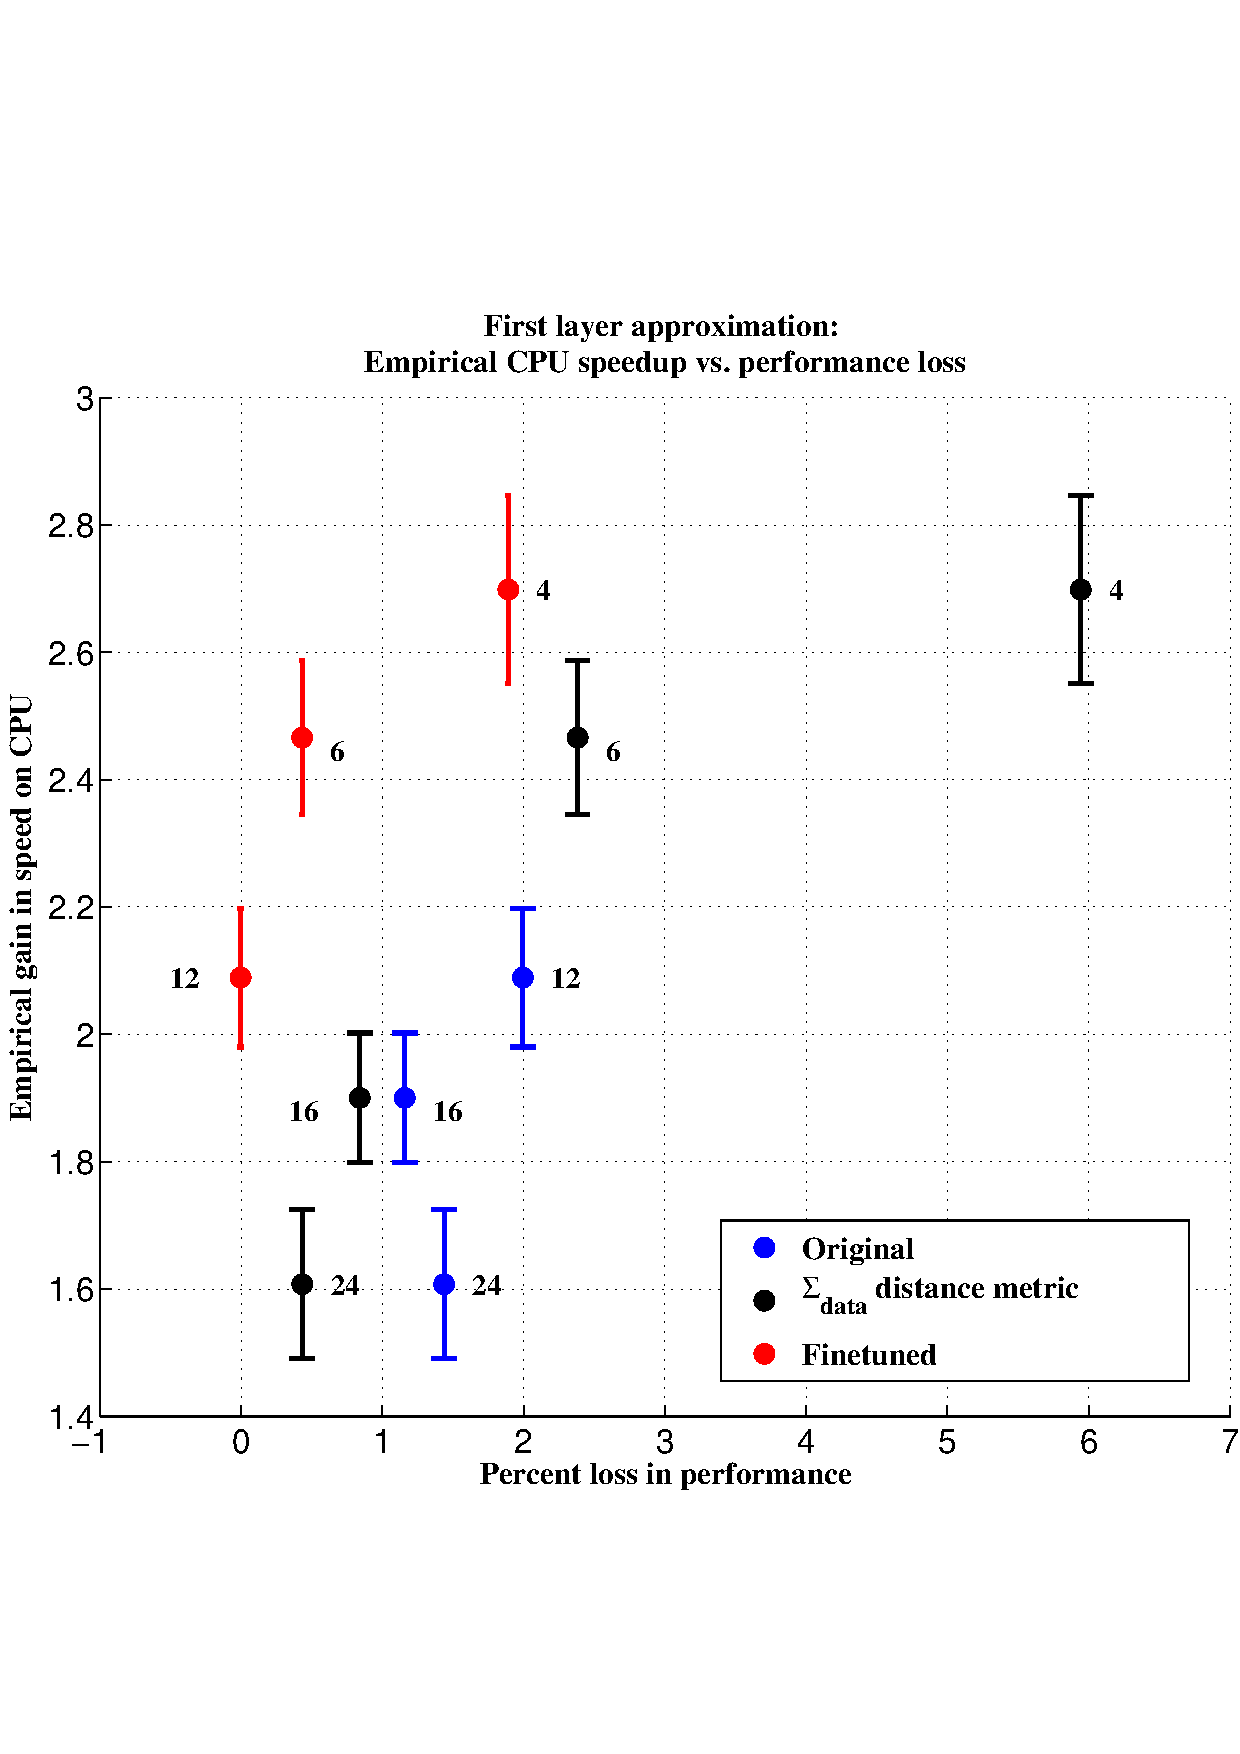
\includegraphics[width=0.5\linewidth]{img/layer1_CPUspeedup_vs_performance_loss_finetune_and_orig.pdf}
	\quad\quad
      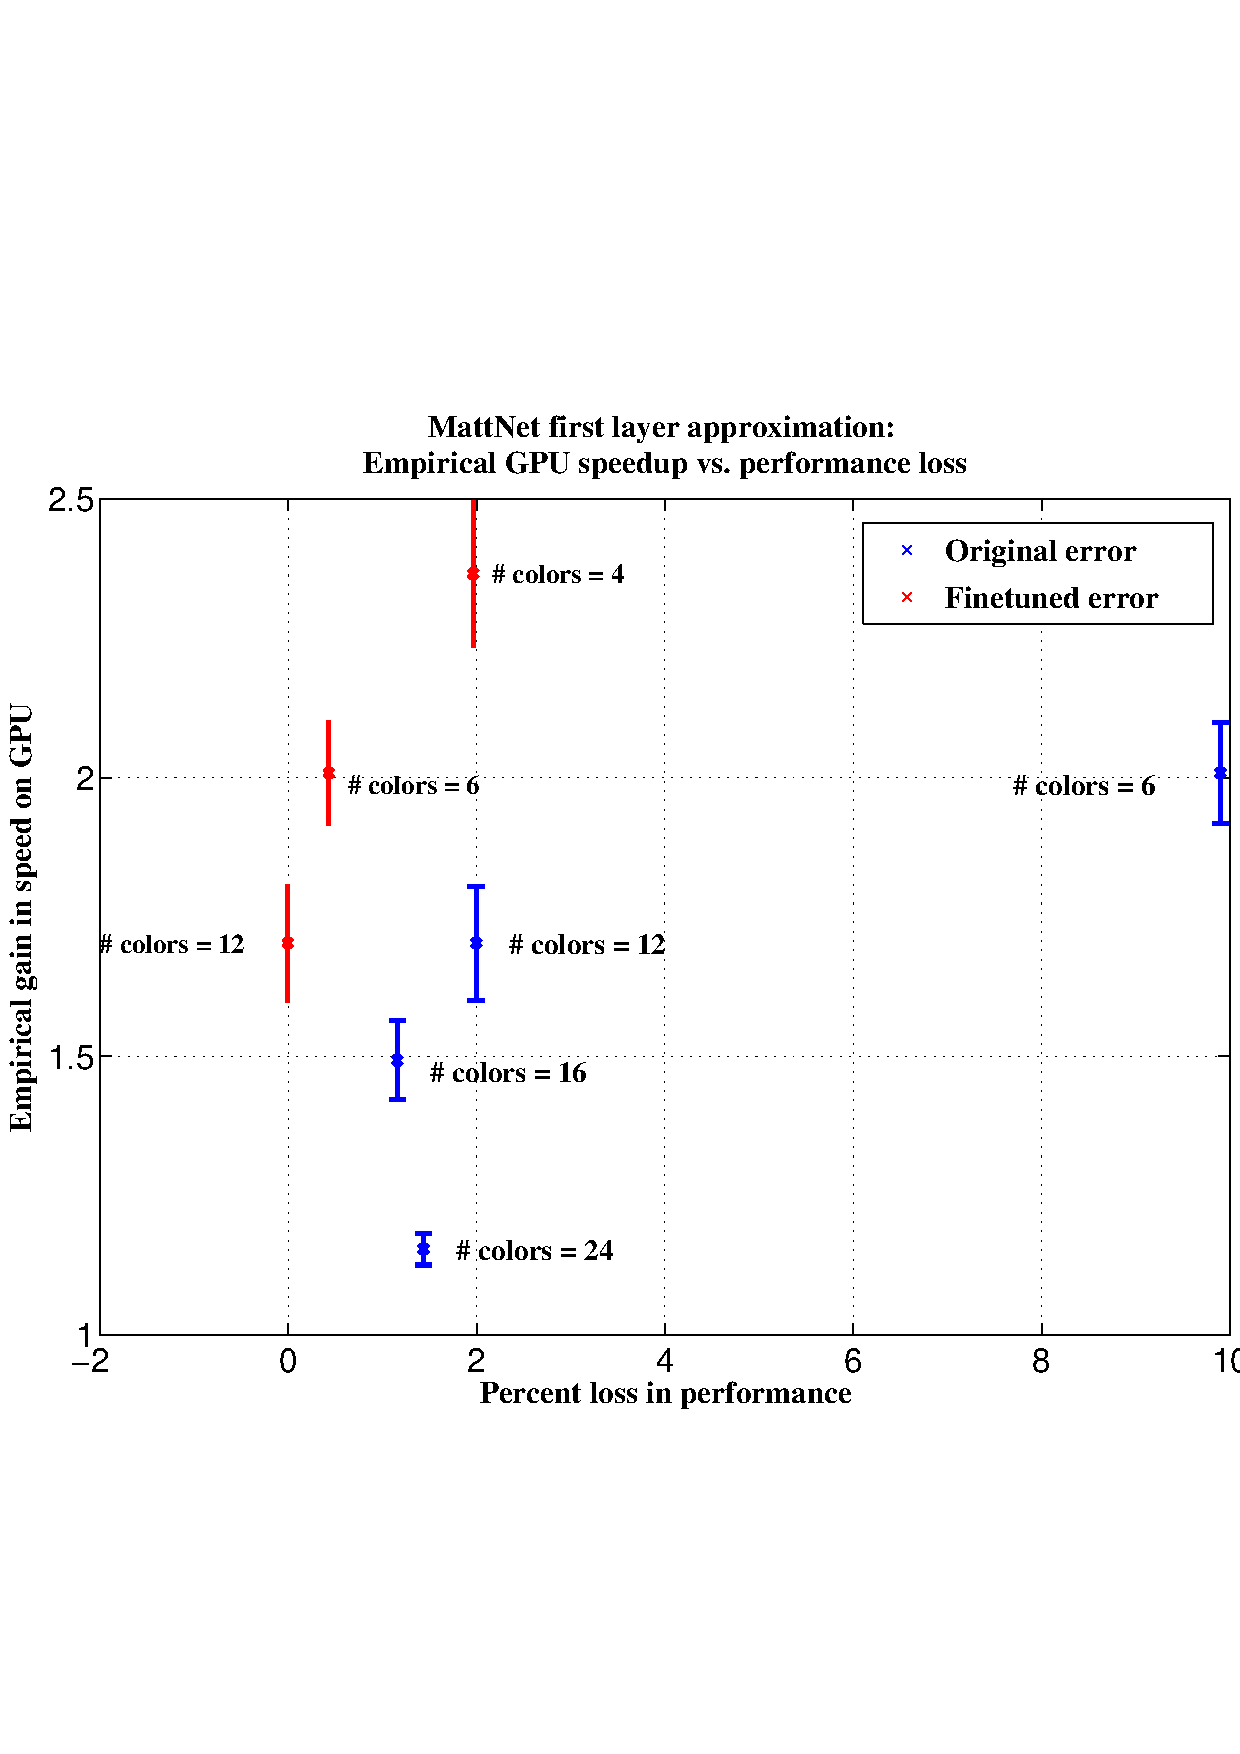
\includegraphics[width=0.5\linewidth]{img/layer1_GPUspeedup_vs_performance_loss_finetune_and_orig.pdf}
\end{minipage}
\caption{Empirical speedups on ({\bf Left}) CPU and ({\bf Right}) GPU for the first layer. $C'$ is the number of colors used in the approximation.}
\label{fig:mono_speedups}
\end{figure}

\subsubsection{Second Layer}
The second convolutional layer has 96 input channels, 256 output channels and 5x5 filters. 
We approximated the weights using the techniques described in section \ref{subsec:clustering}. 
We evaluated the original and approximate convolution operation in
this layer using 20K validation images from the ImageNet12 dataset. 
We explored various configurations of the approximations by varying the number of input clusters $G$, the number of output clusters $H$ and the rank of the approximation (denoted by $K_1$ and $K_2$ for the SVD decomposition and $K$ for the outer product decomposition). 

Figure \ref{fig:biclust_speedups} shows our empirical speedups on CPU
and GPU and the corresponding network performance for
various approximation configurations. For the CPU implementation we used the biclustering with SVD approximation. For the GPU implementation we using the biclustering with outer product decomposition approximation.  
We achieved promising results and present speedups of $2-2.5\times$ relative to the baseline with less than a 1\% drop in performance.

\begin{figure}[t]
\centering
\begin{minipage}{0.9\textwidth}
      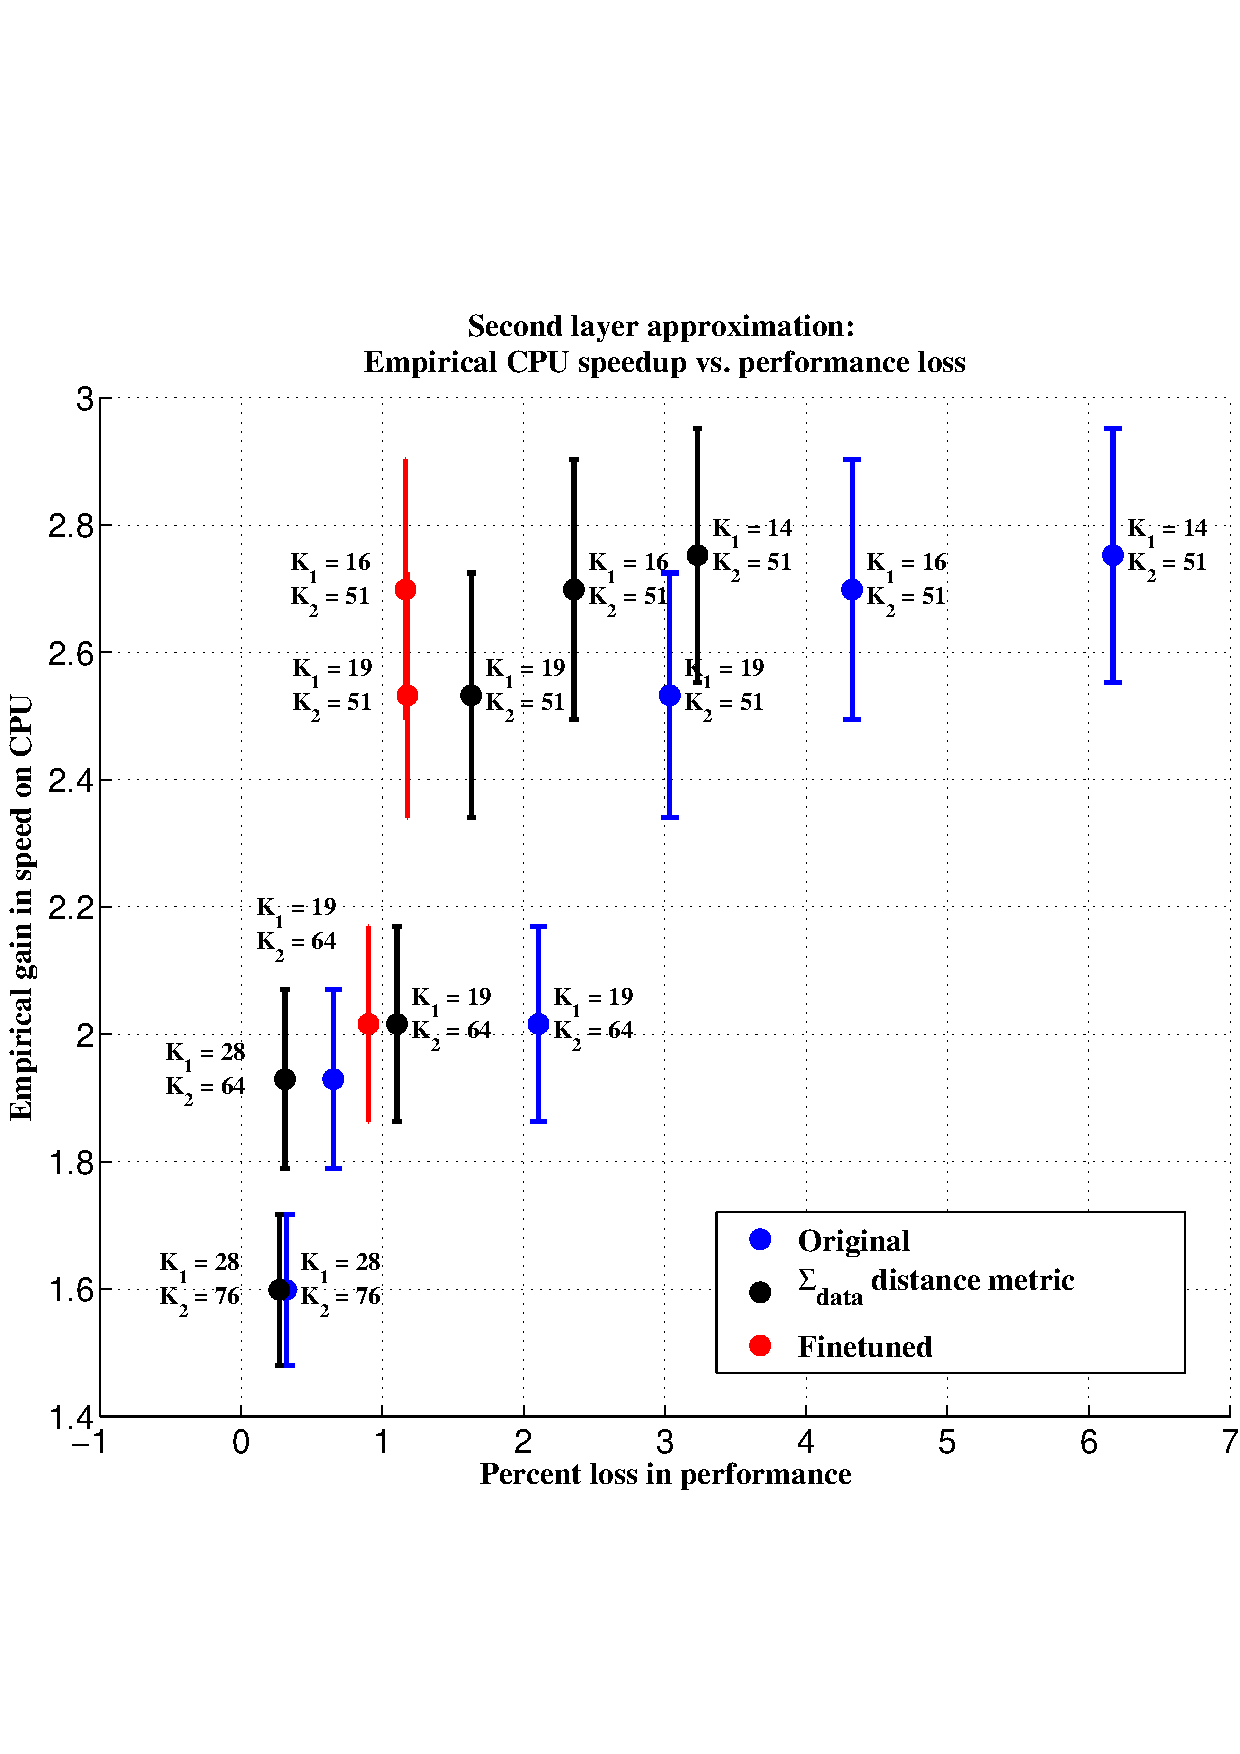
\includegraphics[width=0.5\linewidth]{img/layer2_CPUspeedup_vs_performance_loss_finetune_and_orig.pdf}
      \quad\quad
      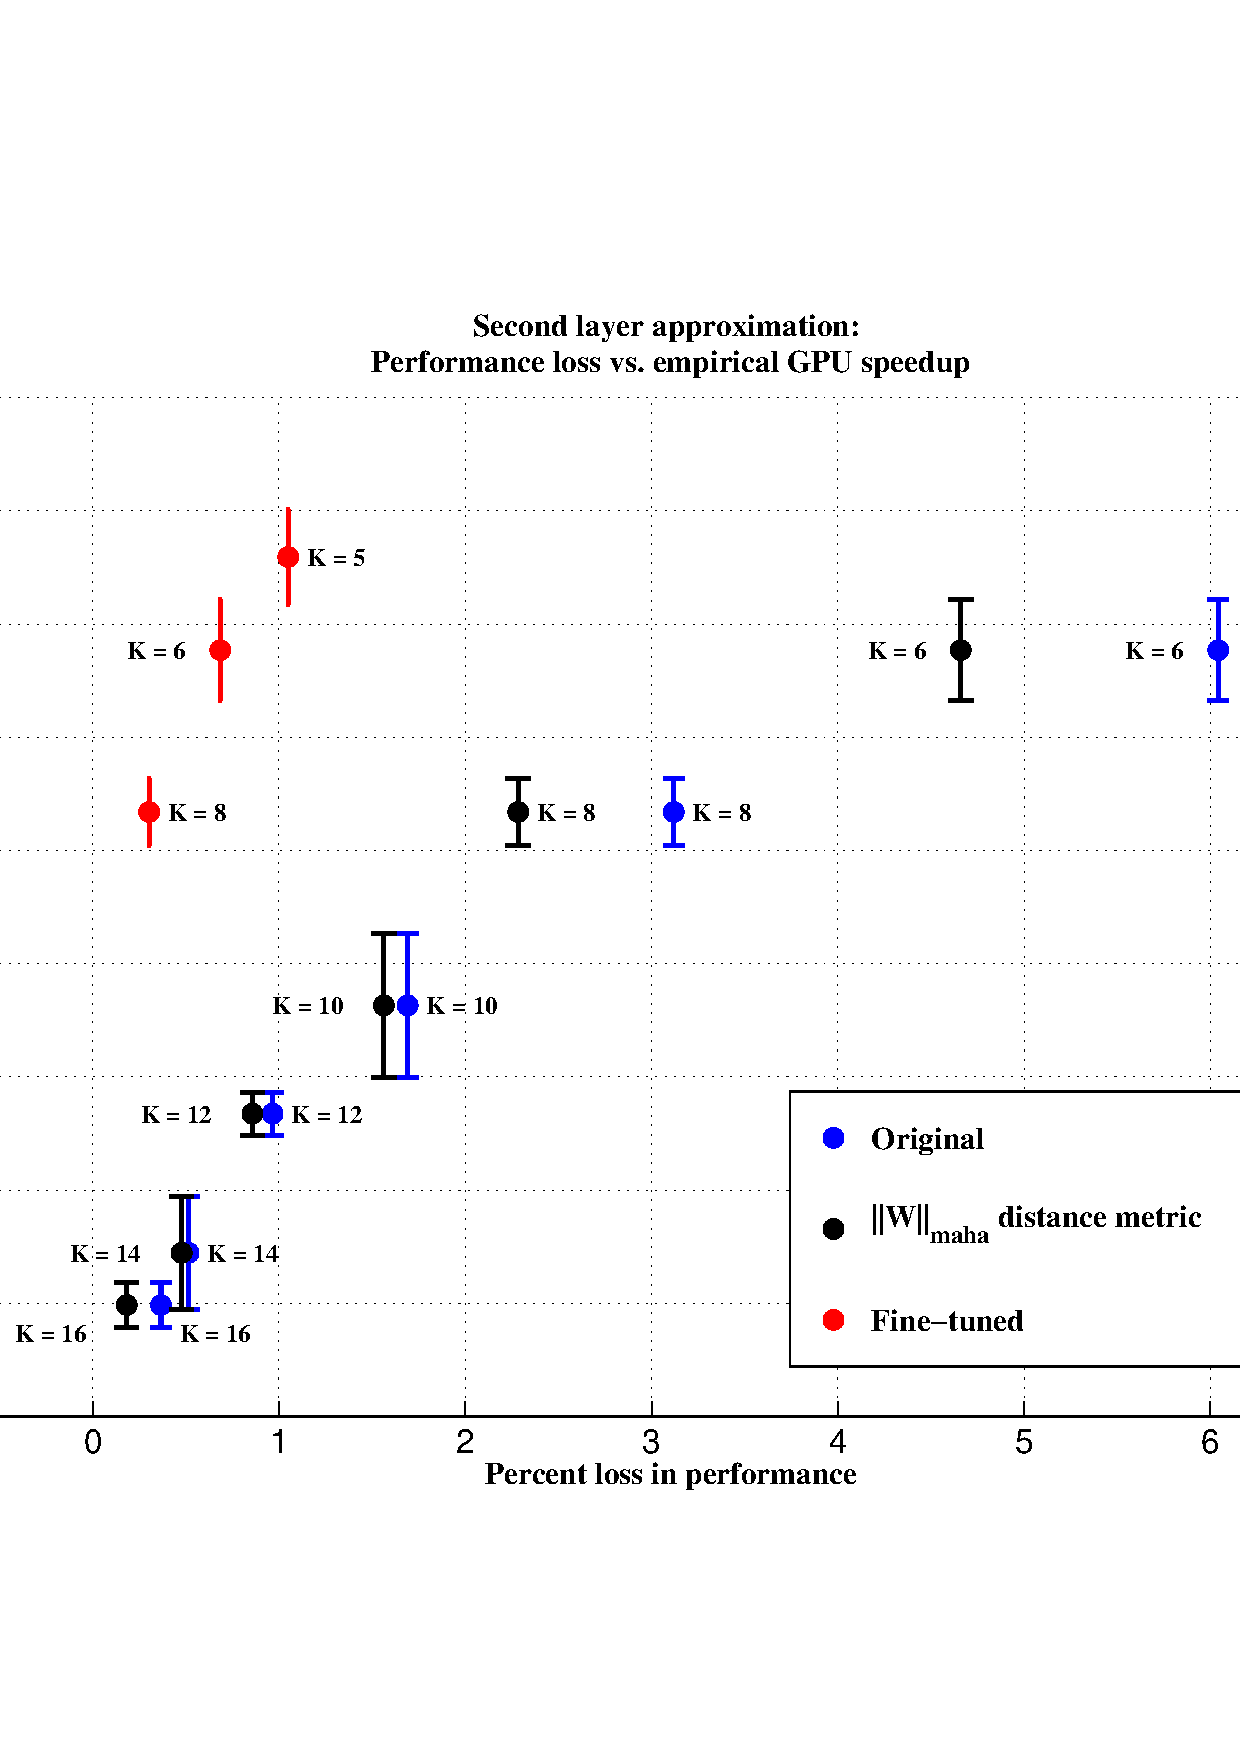
\includegraphics[width=0.5\linewidth]{img/layer2_GPUspeedup_vs_performance_loss_finetune_and_orig.pdf}
\end{minipage}
\caption{Empirical speedups for second convolutional layer. ({\bf Left}) Speedups on CPU using biclustered ($G = 2$ and $H = 2$) with SVD approximation.({\bf Right}) peedups on GPU using biclustered ($G = 48$ and $h = 2$) with outer product decomposition approximation.}
\label{fig:biclust_speedups}
\end{figure}

\subsection{Combining approximations}
The approximations can also be cascaded to provide greater speedups.
The procedure is as follows. 
First, compress the first convolutional layer weights and then fix the layer. 
Fine-tune all the layers above until performance is restored. 
Next, compress the second convolutional layer weights that result form the fine-tuning.
Fine-tune all the layers above until performance is restored and then continue the process. 

We applied this procedure to the first two convolutional layers. 
We used the monochromatic approximation with 6 colors for the first layer approximation. 
We used the biclustering with outer product decomposition approximation for the second layer. 
Fine-tuning with a single pass through the training set resulted in a network whose prediction accuracy was within 1\% of the original model.
This procedure could be applied to each convolutional layer, in this sequential manner, to achieve overall speedups much greater than any individual layer can provide. 

\subsection{Reduction in memory overhead}
In many commercial applications memory conservation and storage are a
central concern. This mainly applies to embedded systems
(e.g. smartphones), where available memory is limited, and users are
reluctant to download large files. In these cases, being able to
compress the neural network is crucial for the viability of the
product. 

In addition to requiring fewer operations, our approximations
require significantly fewer parameters when compared to the original
model. 
Since the majority of parameters come from the fully connected layers, we include these layers in our analysis of memory overhead. We compress the fully connected layers using standard SVD as described in \ref{subsubsec:svd_tensor}. We use $K$ to denote the rank of the approximation.
 
Table \ref{table:memory} shows the number of parameters for
various approximation methods as a function of hyperparameters for the approximation techniques.
The table also shows the empirical reduction of parameters and the corresponding network performance for specific instantiations of the approximation parameters.

\begin{table}[t]
\tiny
\centering
\begin{tabular}{|l|c|c|c|c|}
\hline
{\bf Approximation method} & {\bf Number of parameters} & {\bf Approximation} & {\bf Reduction} & {\bf Increase in}\\ 
& & {\bf hyperparameters} &  {\bf in weights} & {\bf test error}\\
\hline
\hline
Standard colvolution & $CXYF$ & & &\\
\hline
Conv layer 1: Monochromatic & $CC' + XYF$ & $C' = 6$ & $3\times$ & 0.43\%\\
\hline
Conv layer 2: Biclustering & $GHK (\frac{C}{G} + XY + \frac{F}{H})$ & $G = 48$; $H = 2$; $K = 6$ & 5.3$\times$ & 0.68\%\\
	    + outer product decomposition  & &  & &\\
\hline
Conv layer 2: Biclustering + SVD& $G H (\frac{C}{G}K_1 + K_1 X Y K_2 + K_2 \frac{F}{H})$ & $G = 2; H = 2$; $K_1 = 19$; $K_2 = 24$ & $3.9\times$ & 0.9\% \\
\hline
Standard FC & $N M$ & & &\\
\hline
FC layer 1: Matrix SVD & $NK + KM$ & $K = 250$ & $13.4\times$ & 0.8394\%\\
                      & & $K = 950$ & $3.5\times$ & 0.09\%\\
\hline 
FC layer 2: Matrix SVD & $NK + KM$ & $K = 350 $ & $5.8\times$ & 0.19\%\\
                      & & $K = 650$ & $3.14\times$ & 0.06\%\\
\hline 
FC layer 3: Matrix SVD & $NK + KM$ & $K = 250$ & $8.1\times$ & 0.67\%\\
                      & & $K = 850$ & $2.4\times$ & 0.02\%\\
\hline 
\end{tabular}
\caption{Number of parameters expressed as a function of hyperparameters for various approximation methods and empirical reduction in parameters with corresponding network performance.} 
\label{table:memory}
\end{table}
\vspace{-3mm}


\section{Discussion}

In this paper we have presented techniques that can speed up the
bottleneck convolution operations in the first layers of a convolutional network by a factor $1.6-2$, with a
moderate loss of performance ($\sim1\%$). The empirical speedups
achieved are still some way short of the theoretical gains, thus
further improvements might be expected with further engineering effort. 
Moreover, the techniques are orthogonal
to other approaches for efficient evaluation, such as quantization or
working in the Fourier domain. Hence, they can potentially be used
together to obtain further gains. 

Given the widespread use of neural networks in large scale industrial
settings, the speed gains we demonstrate have significant economic
value. Companies such as Google or Facebook process $10^8$ images/day,
requiring many thousands of machines. Our speed gains mean that the
number of machines dedicated to running convolutional networks could be roughly halved, so saving millions of
dollars, as well as a significant reduction in environmental impact.


We also show that our methods reduce the memory footprint of weights
in the first two layers by factor of $2-3\times$. When applied to the whole network,
this would translate into a significant savings, which would facilitate mobile deployment
of convolutional networks.

Our approximations are applied to fully trained networks. The
small performance drops that result could well be mitigated by further
training the network after applying the approximation. By alternating
these two steps, we could potentially achieve further gains in
speed-up for a modest performance drop.


Another aspect of our technique is regularization. It seems that
approximated filters look cleaner, and that sporadically we get better
test error (e.g.~bottom left of Figure
\ref{fig:biclustering_theory}(left)). We would like to experiment with
low-rank projections during training as a regularization
technique. Effectively it decreases number of learnable parameters,
so it might improve generalization, a major issue with large convolutional networks.
  


% Presented methods were applied to fully trained networks. Obviously, networks were not trained
% with constrains on connectivity or sparsity as are present in approximated network. This means 
% that agresive approximations, which can have much larger speedup are likely to give worse error score. 
% Training with new connectivity or sparsity constraint might be quite difficult. Constrains 
% comming from approximation would have to be included in optimization, and a lot of additional coding would be
% neccessary. We propose different strategy. 


% It is easy to decompose weights using any of our method, and then reconstruct them. Particularly,
% reconstructed weights can be approximated exactly with the same decomposition. Let's call this process
% projection. Proposed strategy is to take a fully trained network, and iterativelly repeat (1) apply projection, 
% (2) train for few epochs. Hopefuly, this way weights will become expressable in desired way, which can be speededup
% more than $2$ times, and prediction score would be preserved due to fine-tunning. From engineering perspective
% stage (1) can be implemented in any external easy environment (e.g. MATLAB), while stage can stay as it is. 
% Stage (1) is executed every few epochs, so it is not a computational bottle-neck.



% and thus our speed gains 

% the speed gains we demonstrate have 
% Speeding up the evaluation of neural networks has a high industrial impact. Computation
% of forward pass on all public internet available images (billions of images), or
% on all social media data cost in milions of dollars for a single pass. High costs
% of evaluation limits use of neural networks, and might forces companies to rely
% on inferior object recognition techniques which are much cheaper in evaluation 
% (e.g. SIFT features). 



% Presented in this paper techniques show how to achieve speedup by the factor of $2$,
% with moderate loss of performance ($< 1\%$). Moreover, they are ortogonal 
% to previously developed techniques like quantization, or working in Fourier domain, and
% can be used together to further boost evaluation speed. Finally, we believe that fine-tunning
% technique described in Section \ref{sec:fine_tunning} can enable even further 
% agresive approximations, and give a higher boost.



%\subsection{Fine-tunning}\label{sec:fine_tunning}

Presented methods were applied to fully trained networks. Obviously, networks were not trained
with constrains on connectivity or sparsity as are present in approximated network. This means 
that agresive approximations, which can have much larger speedup are likely to give worse error score. 
Training with new connectivity or sparsity constraint might be quite difficult. Constrains 
comming from approximation would have to be included in optimization, and a lot of additional coding would be
neccessary. We propose different strategy. 


It is easy to decompose weights using any of our method, and then reconstruct them. Particularly,
reconstructed weights can be approximated exactly with the same decomposition. Let's call this process
projection. Proposed strategy is to take a fully trained network, and iterativelly repeat (1) apply projection, 
(2) train for few epochs. Hopefuly, this way weights will become expressable in desired way, which can be speededup
more than $2$ times, and prediction score would be preserved due to fine-tunning. From engineering perspective
stage (1) can be implemented in any external easy environment (e.g. MATLAB), while stage can stay as it is. 
Stage (1) is executed every few epochs, so it is not a computational bottle-neck.






%\subsubsection*{Acknowledgments}

\nocite{*}
\bibliographystyle{splncs}
\bibliography{bibliography}

\end{document}
